\documentclass{term-paper}

\usepackage{setup}

\title{Оцінка ефективності алгоритмів}
\author{Черних О. Ф.}
\date{2026}

\begin{document}

\begin{titlepage}
    \begin{center}
        {\fontshape{sc}\selectfont МІНІСТЕРСТВО ОСВІТИ І НАУКИ УКРАЇНИ} \\
        \vspace{0.5cm}
        Національний аерокосмічний університет
        \\ \enquote{Харківський авіаційний інститут}
        \vspace{0.5cm}
        \\ Факультет літакобудування
        \vspace{0.5cm}
        \\ Кафедра інформаційних технологій проєктування
    \end{center}
    \vspace{2.0cm}
    \begin{center}
        {\Large\textbf{\thetitle}\par}
        \vspace{0.5cm}
        \small{З курсу: \enquote{Обробка та аналіз результатів НД з використанням ІТ}\par}
    \end{center}
    \vspace{3.0cm}
    \hfill\parbox{7.0cm}{
        \begin{flushleft}
            \textbf{Виконав}\\
            \theauthor
        \end{flushleft}}
    \vfill

    \begin{center}
        Харків -- \thedate
    \end{center}
\end{titlepage}


\section*[Звіт]{ЗВІТ}

\section{Методика тестування}

Весь вихідний код проєкту доступний у репозиторії GitHub:\\
\url{https://github.com/uspiritwolf/sort-benchmark}.

\par Для вимірювань використано бібліотеку Google Benchmark~v1.9.5, яку
підключено до проєкту засобами CMake (\texttt{FetchContent}). Програма
написана мовою C++23 і зібрана компілятором Clang зі стандартною бібліотекою
libc++ у конфігурації Release. Вимірювання виконано на процесорі з 16
логічними ядрами (5{,}26~ГГц), L1 даних 32~КіБ на ядро, L2 1~МіБ на ядро,
L3 16~МіБ.

Досліджено 13 алгоритмів сортування масиву цілих чисел \texttt{int}:
сортування бульбашкою, гномове, пірамідальне, вставками, introsort, злиттям,
швидке, порозрядне (radix), вибором, Шелла, сортування деревом
(\texttt{std::multiset}), а також бібліотечні \texttt{std::sort} для
\texttt{std::vector} і \texttt{std::list::sort}. Кожен алгоритм
перевірявся на трьох типах вхідних даних:
\begin{itemize}
    \item \emph{random} --- випадкові значення від генератора
          \texttt{std::mt19937};
    \item \emph{sorted} --- уже відсортована послідовність $0, 1, \dots, N-1$;
    \item \emph{reverse-sorted} --- послідовність, відсортована у зворотному
          порядку.
\end{itemize}

Розмір вхідних даних $N$ починається зі 128 і подвоюється на кожному
кроці. Верхня межа обрана так, щоб тест виконувався за прийнятний час:
4096 для квадратичних алгоритмів (бульбашка, вибір, а також вставки та
гномове сортування на random і reverse-sorted), 65\,536 для більшості
інших і 262\,144 для порозрядного сортування.

Кожен тест складається з трьох частин. Перша --- спільна для всіх типів
даних обгортка (лістинг~\ref{lst:run}). У циклі \texttt{for (auto \_ : state)}
бібліотека сама визначає кількість ітерацій, потрібну для стабільного
результату. Копіювання вхідного масиву виконується між
\texttt{PauseTiming()} та \texttt{ResumeTiming()}, тому до виміряного часу
потрапляє лише саме сортування. Коректність результату перевіряє
\texttt{assert}. Виклик \texttt{SetComplexityN()} повідомляє бібліотеці
розмір задачі $N$, який далі використовується для оцінки складності.

\begin{listing}[H]
    \begin{minted}{cpp}
void run_radix_sort(benchmark::State& state, const std::vector<int>& data)
{
    for (auto _ : state)
    {
        state.PauseTiming();
        std::vector<int> data_copy(data);
        state.ResumeTiming();

        radix_sort(data_copy.begin(), data_copy.end());
        assert(std::ranges::is_sorted(data_copy));
    }

    state.SetComplexityN(state.range(0));
}
\end{minted}
    \caption{Обгортка вимірювання (на прикладі порозрядного сортування)}
    \label{lst:run}
\end{listing}

Друга частина --- функції, що готують вхідні дані кожного типу: масив
довжини \texttt{state.range(0)} заповнюється випадковими числами
(\texttt{std::mt19937}), зростаючою послідовністю (\texttt{std::ranges::iota})
або спадною (\texttt{iota} у зворотному порядку), після чого передається в
обгортку з лістингу~\ref{lst:run}.

Третя частина --- реєстрація тестів макросом \texttt{BENCHMARK}
(лістинг~\ref{lst:register}). Виклики \texttt{RangeMultiplier(2)}
і~\texttt{Range(128,~262144)} задають геометричну послідовність
розмірів $N = 128, 256, \dots, 262\,144$, а~виклик \texttt{Complexity()}
вмикає
автоматичну оцінку асимптотичної складності за результатами всіх
розмірів.

\begin{listing}[H]
    \begin{minted}{cpp}
BENCHMARK(radix_sort_random)
    ->RangeMultiplier(2)
    ->Range(128, 262144)
    ->Complexity();

BENCHMARK(radix_sort_sorted)
    ->RangeMultiplier(2)
    ->Range(128, 262144)
    ->Complexity();

BENCHMARK(radix_sort_reverse_sorted)
    ->RangeMultiplier(2)
    ->Range(128, 262144)
    ->Complexity();
\end{minted}
    \caption{Реєстрація тестів з оцінкою складності}
    \label{lst:register}
\end{listing}

Для решти алгоритмів тести побудовано так само, змінюються лише функція
сортування та верхня межа $N$. Усі тести запущено одним викликом програми
з вивантаженням результатів у CSV. В аналізі використано процесорний час
(CPU time) на одну ітерацію в наносекундах.

\section{Оцінка складності засобами Google Benchmark}

Google Benchmark може сам оцінити асимптотичну складність (Big-O) за
виміряними даними. Якщо викликати \texttt{Complexity()} без аргументів
(режим \texttt{oAuto}), бібліотека по черзі перебирає класи $O(1)$,
$O(\log N)$, $O(N)$, $O(N \log N)$, $O(N^2)$ і $O(N^3)$. Для кожного класу
вона методом найменших квадратів підбирає коефіцієнт $c$ у моделі
\begin{equation}
    t(N) \approx c \cdot f(N)
\end{equation}
де $t(N)$ --- час виконання для вхідних даних розміру $N$;\\
$c$ --- сталий коефіцієнт, який бібліотека підбирає за виміряними даними;\\
$f(N)$ --- функція зростання для перевірюваного класу складності
(наприклад, $N$, $N \log N$ або $N^2$).

Бібліотека обирає клас з найменшою похибкою апроксимації. До результатів кожної
серії бібліотека додає два рядки: \texttt{\_BigO} з коефіцієнтом і класом
(наприклад, \texttt{0.45~NlgN}) та \texttt{\_RMS} з похибкою підбору.

Отримані класи складності наведено на рисунку~\ref{fig:complexity}.
Зеленим позначено очікувано добрий результат: для random і reverse-sorted
це клас не гірший за $O(N \log N)$, а для вже відсортованих даних --- не
гірший за $O(N)$. Жовтим позначено решту субквадратичних класів (наприклад,
$O(N \log N)$ на відсортованих даних), червоним --- $O(N^2)$ і гірші.

\begin{figure}[H]
    \centering
    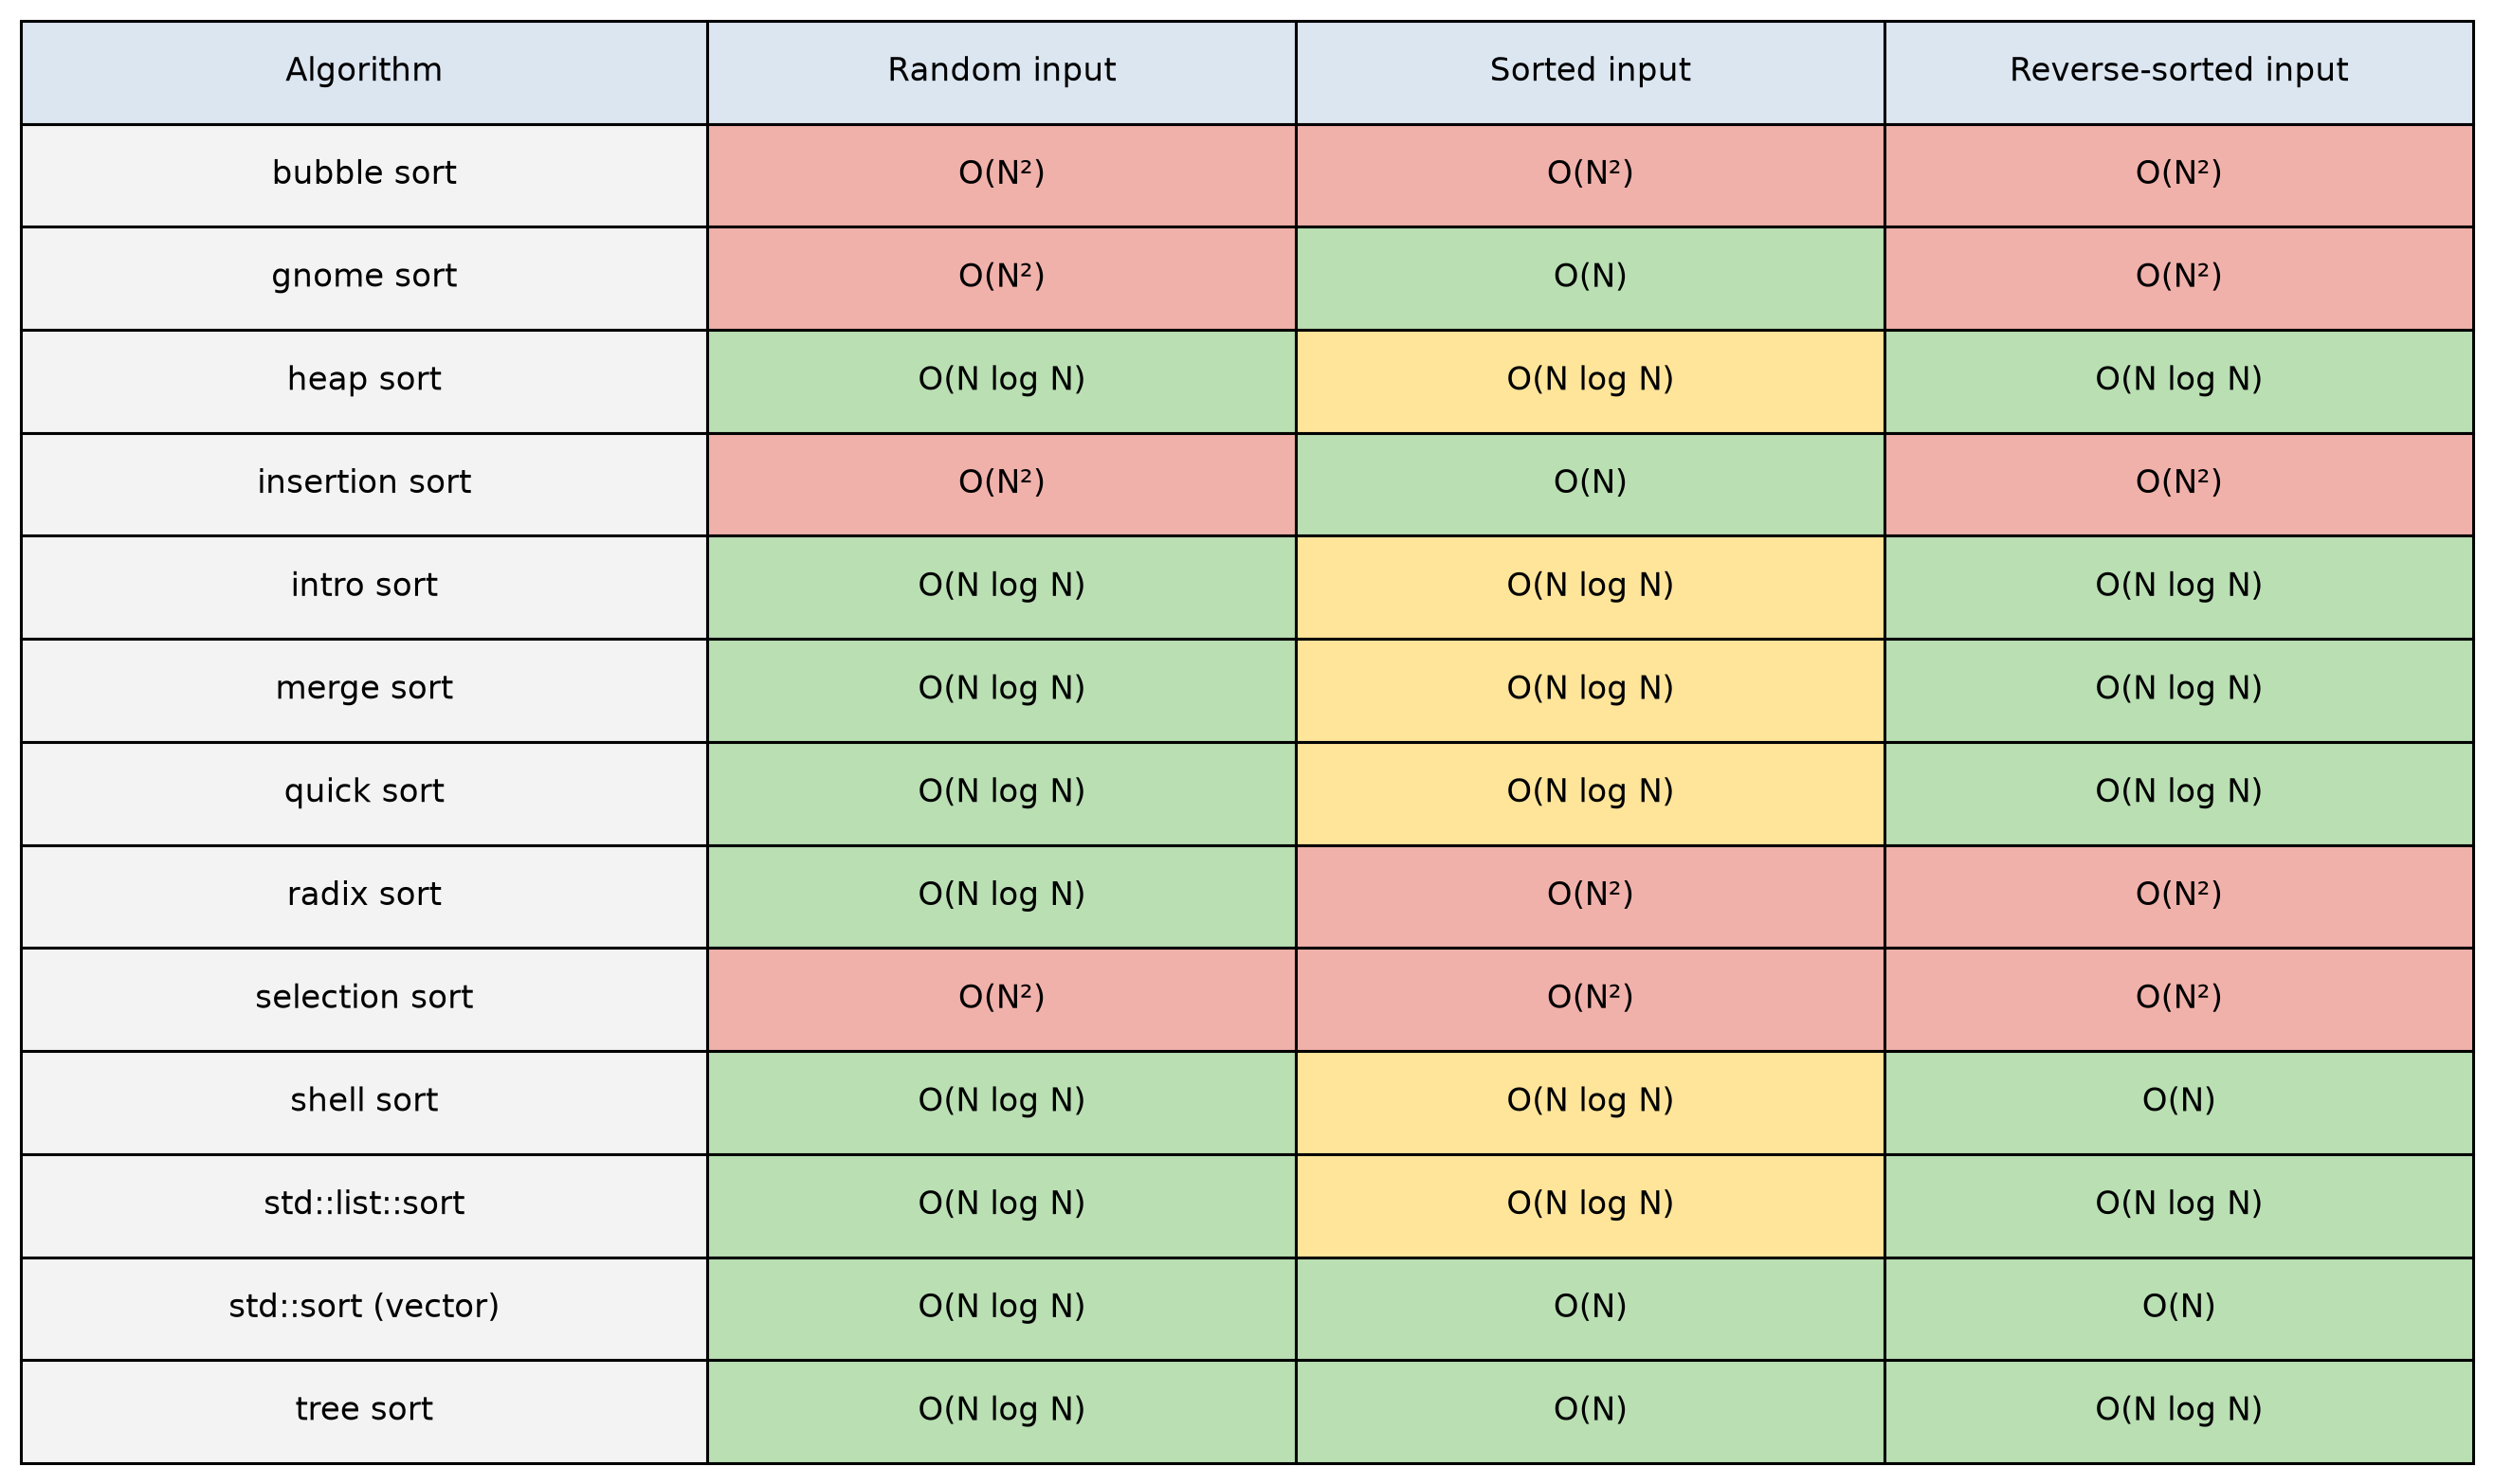
\includegraphics[width=\linewidth]{result/benchmark_complexity.png}
    \caption{Класи складності, оцінені Google Benchmark, для кожного
        алгоритму та типу вхідних даних}
    \label{fig:complexity}
\end{figure}

Здебільшого оцінки збігаються з теоретичними. Сортування бульбашкою та
вибором квадратичні на всіх типах даних. Сортування вставками та гномове
квадратичні на random і reverse-sorted, але лінійні на відсортованому
масиві, бо там кожен елемент лише один раз порівнюється із сусіднім.
Пірамідальне, introsort, злиттям, швидке сортування та
\texttt{std::list::sort} на всіх типах даних мають $O(N \log N)$.
Сортування деревом отримало $O(N)$ лише на відсортованих даних, а на
інших --- $O(N \log N)$. \texttt{std::sort} на випадкових даних також має
$O(N \log N)$, але на відсортованих отримав оцінку $O(N)$. Це пояснюється
оптимізацією в libc++: якщо під час розбиття масиву не довелося
переставити жодного елемента, бібліотека перевіряє обидві частини
обмеженим сортуванням вставками. Якщо частини вже впорядковані, подальший
поділ не виконується, тому для відсортованого масиву залишається лише
кілька лінійних проходів. На зворотно відсортованих даних Google Benchmark
також оцінив \texttt{std::sort} як $O(N)$, проте пояснити це тим самим
механізмом за наявними даними неможливо, тому це варто розглядати лише як
виміряний результат. Помітний виняток --- порозрядне
сортування, яке розглянуто в наступному розділі.

\newpage
\section{Похибка оцінки складності}

Google Benchmark обирає клас складності лише з фіксованого набору відомих
класів, тому для деяких серій оцінка може бути неточною. Наприклад,
порозрядне сортування теоретично має складність $O(N)$, але на sorted і
reverse-sorted даних бібліотека оцінила його як $O(N^2)$: на найбільших
розмірах час зростає швидше за лінійний через ефекти кешу процесора.

Тому разом із класом складності бібліотека обчислює похибку апроксимації
RMS (нормоване середньоквадратичне відхилення виміряного часу від
підібраної моделі). Чим більше значення, тим гірше обраний клас описує
виміри. Значення похибки для всіх серій наведено на рисунку~\ref{fig:rms};
для порозрядного сортування на sorted і reverse-sorted даних вона
найбільша (16--17\,\%).

\begin{figure}[H]
    \centering
    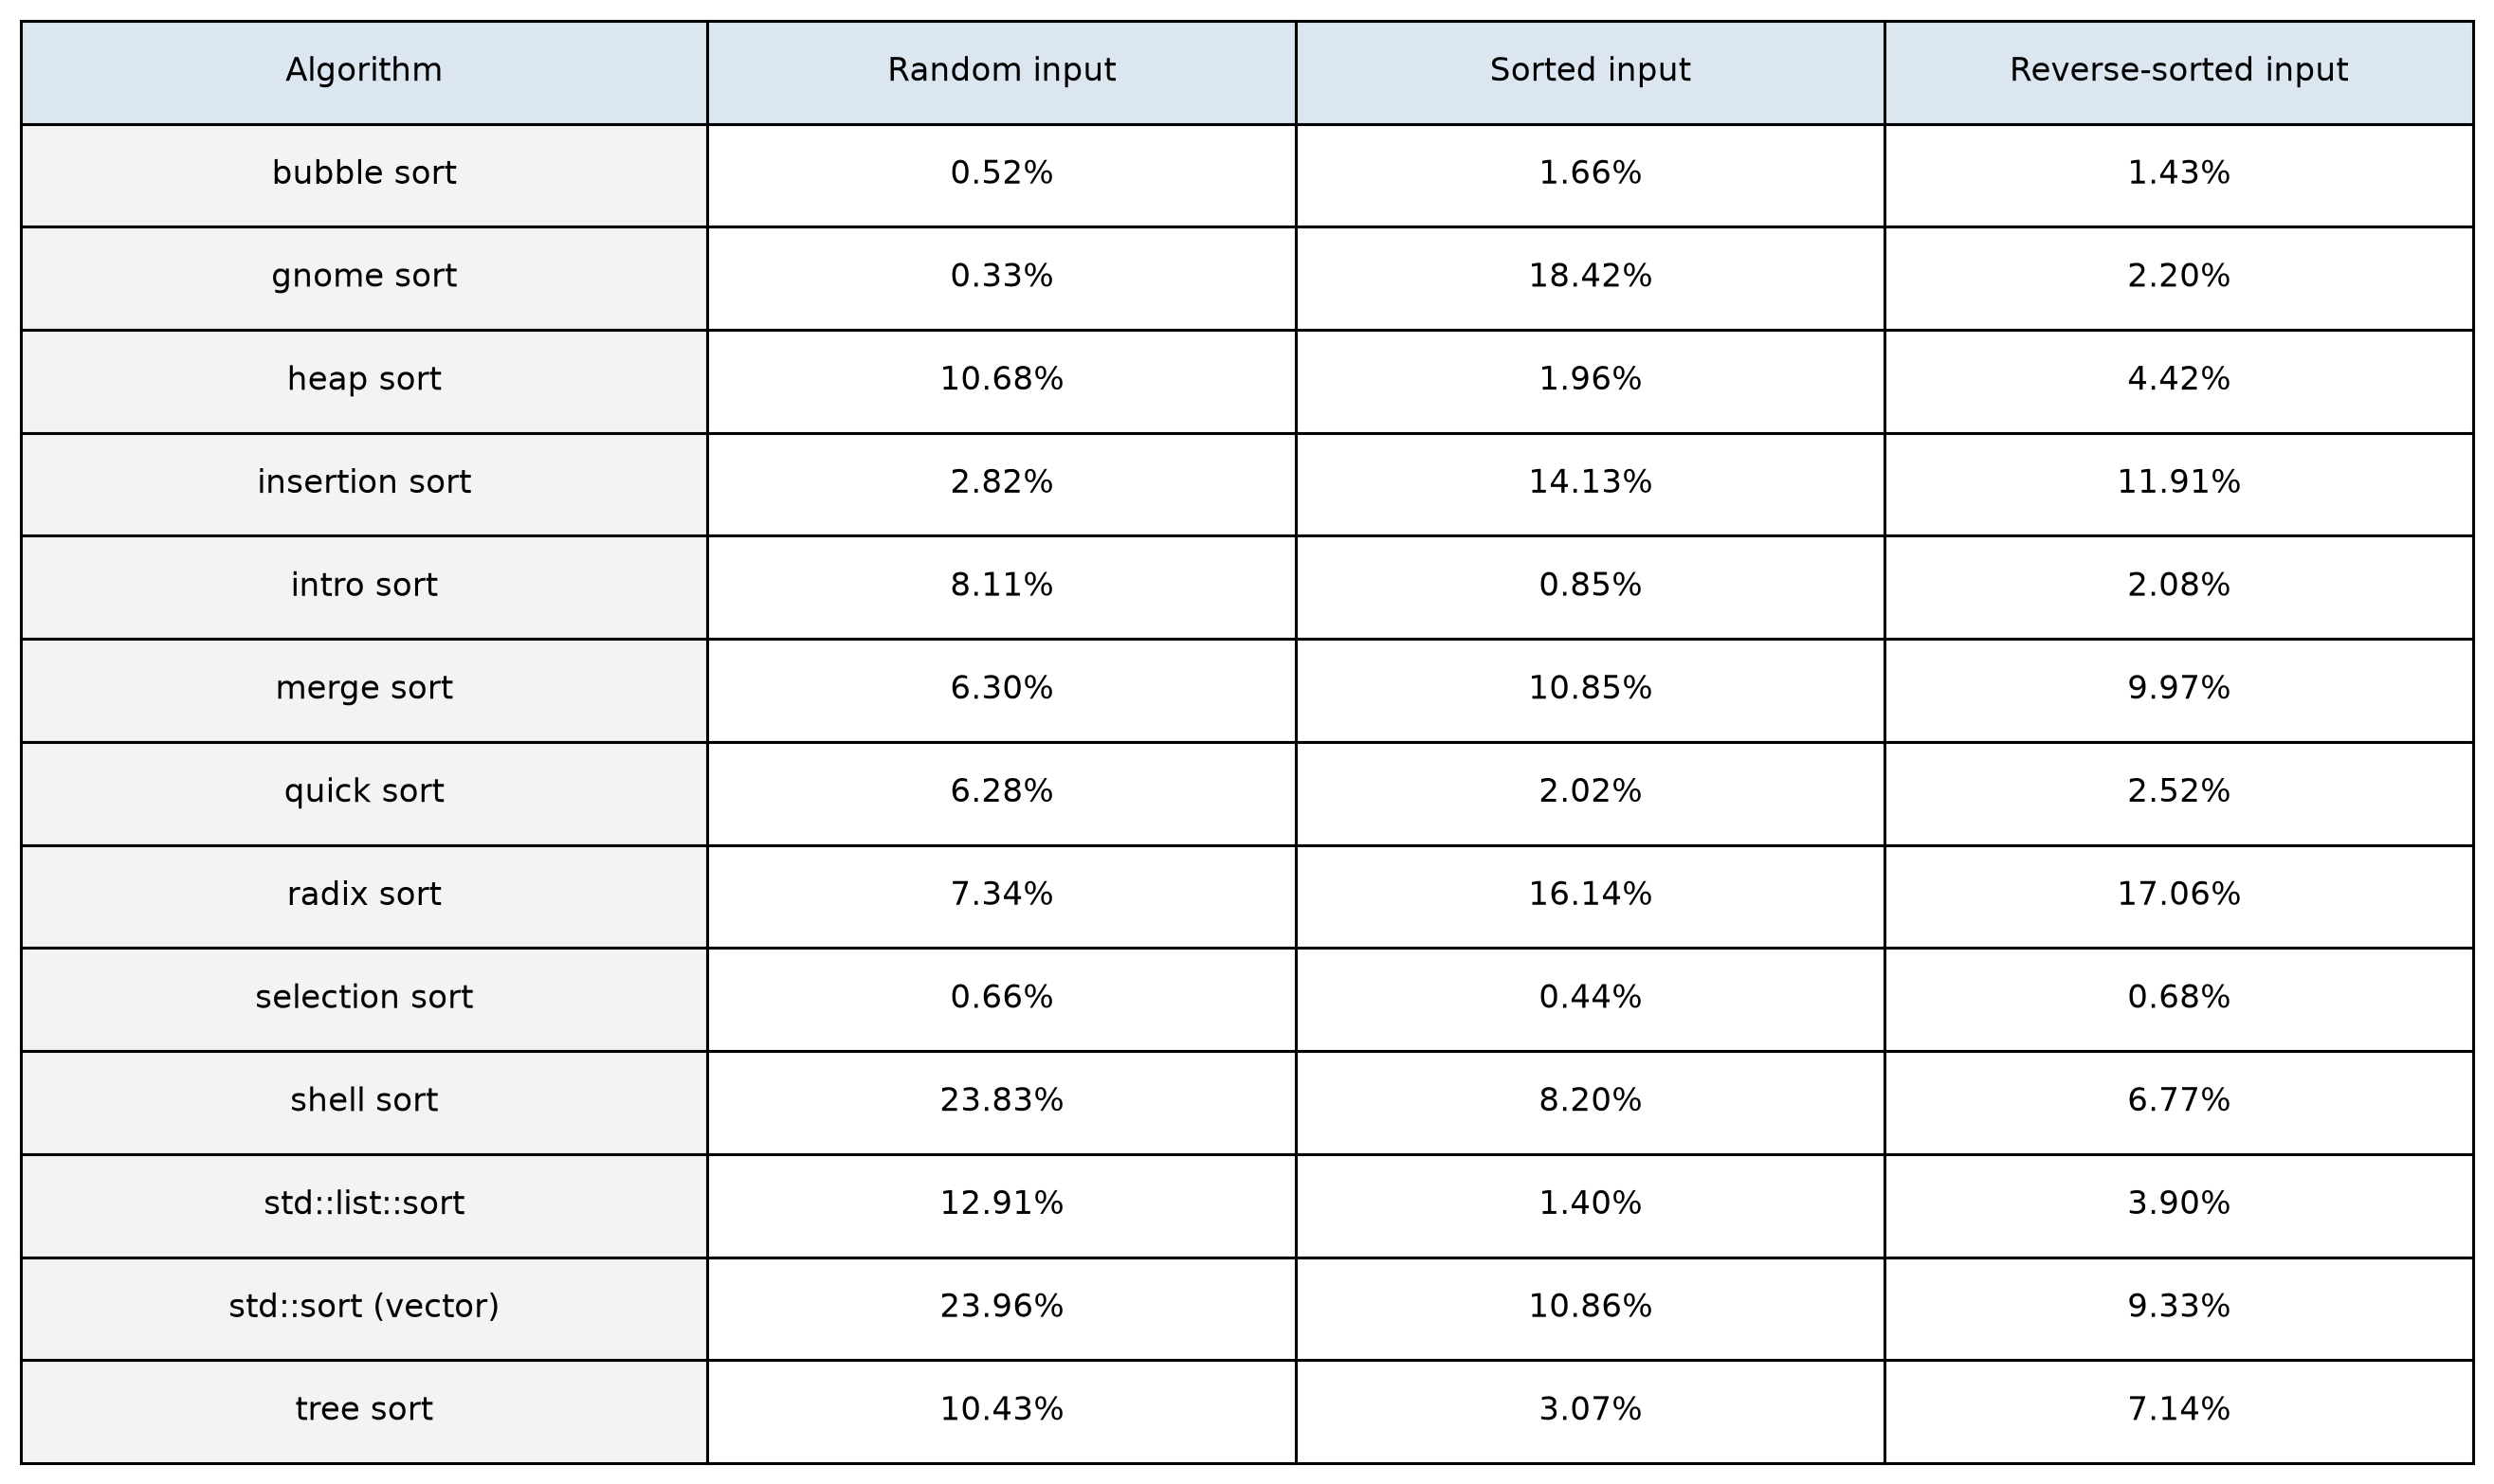
\includegraphics[width=\linewidth]{result/benchmark_rms.png}
    \caption{Похибка RMS оцінки класу складності}
    \label{fig:rms}
\end{figure}

\newpage
\section{Загальний огляд результатів сортування}

Для кожного типу вхідних даних наведено CPU time всіх алгоритмів на
лінійних і логарифмічних шкалах. Усі графіки охоплюють спільний діапазон
$N=128$--$4096$: більші розміри не показані, оскільки частина серій
закінчується на $N=4096$. Лінійні шкали показують абсолютну різницю в часі,
а логарифмічні дають змогу розрізнити алгоритми з дуже різним часом
виконання та порівняти темпи його зростання. Лінії лише з'єднують виміряні
точки. Класи складності в легендах оцінено Google Benchmark за повними
серіями вимірювань, а не лише за показаним діапазоном.

\subsection{Випадкові дані (random)}

На лінійному графіку (рис.~\ref{fig:random-linear}) найбільший час мають
гномове сортування, сортування вибором і бульбашкою. При $N=4096$ він
становить приблизно 5{,}91 мс, 5{,}33 мс і 4{,}10 мс відповідно.
Сортування вставками швидше за ці три алгоритми (1{,}57 мс), але також
помітно відстає від решти. Зі збільшенням $N$ розрив між цією групою та
швидшими алгоритмами зростає.

\begin{figure}[H]
    \centering
    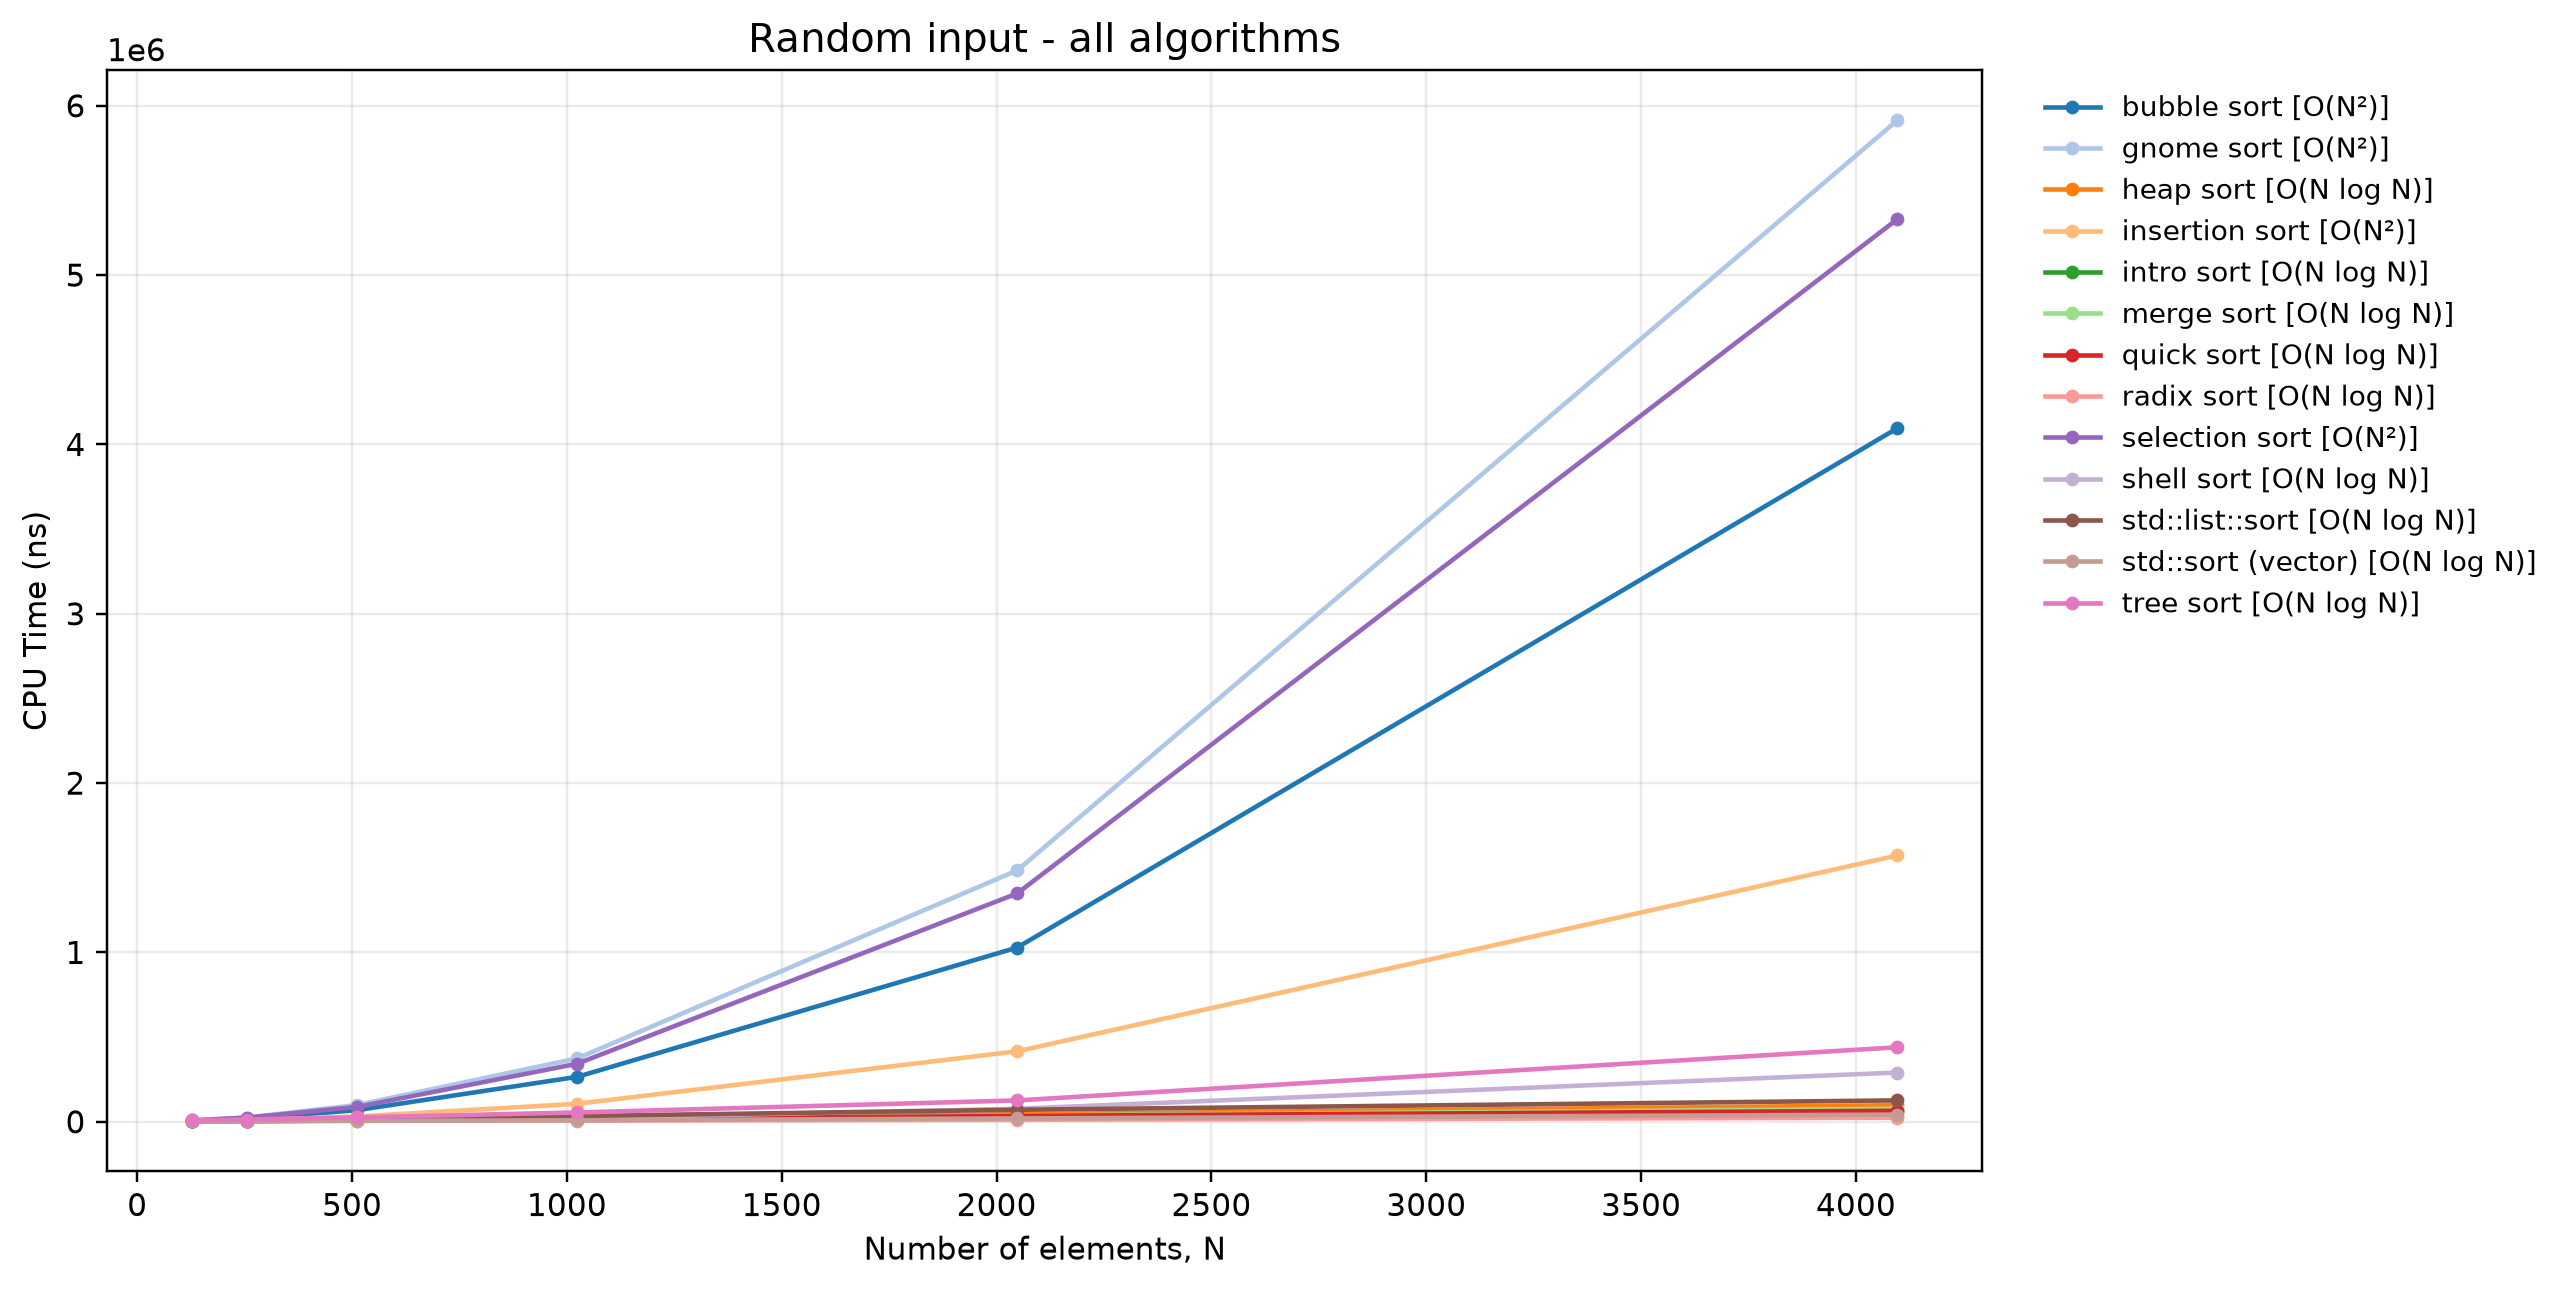
\includegraphics[width=\linewidth]{result/benchmark_overview_random_linear.png}
    \caption{\centering{Час сортування випадкових даних на лінійних шкалах;\\спільний діапазон вимірювань $N=128$--$4096$}}
    \label{fig:random-linear}
\end{figure}

Логарифмічний графік (рис.~\ref{fig:random-loglog}) краще показує відмінності
між швидшими алгоритмами. При $N=4096$ найменший час мають порозрядне
сортування (приблизно 24 мкс) і \texttt{std::sort} для вектора (42 мкс).
Introsort, швидке сортування та сортування злиттям утворюють близьку за
часом групу. Сортування деревом і Шелла в цій точці повільніші за них,
хоча в легенді для всіх цих алгоритмів наведено однакову оцінку
$O(N \log N)$. Отже, однаковий оцінений клас складності не означає
однакового часу виконання.

\begin{figure}[H]
    \centering
    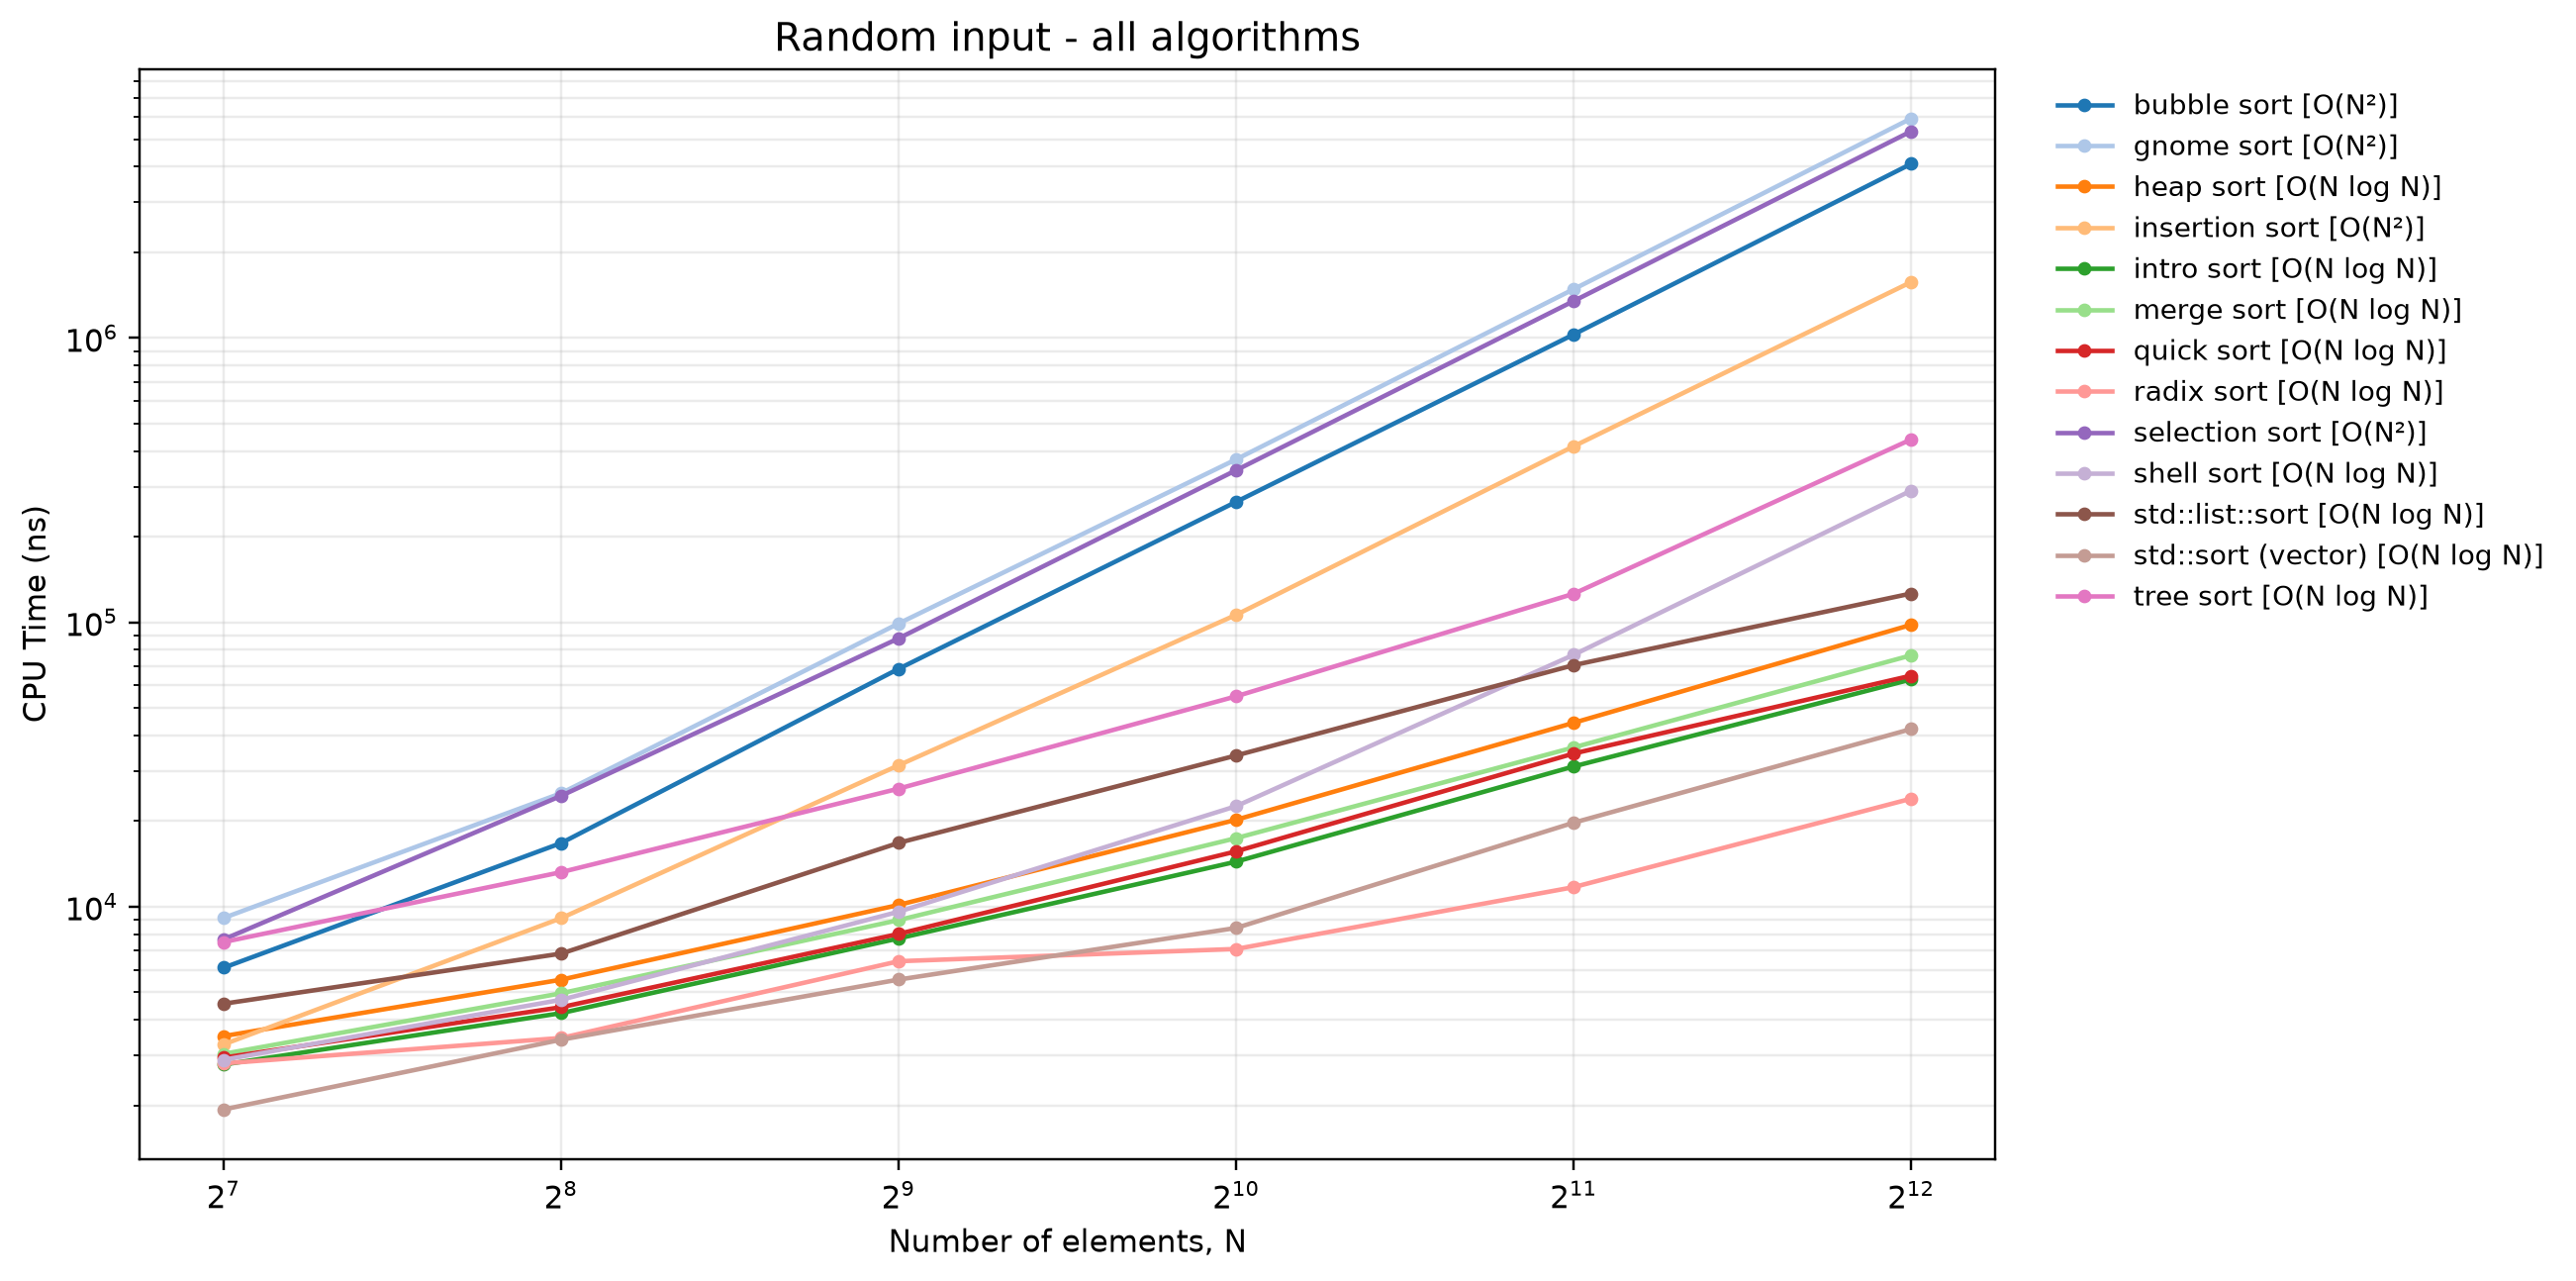
\includegraphics[width=\linewidth]{result/benchmark_overview_random_loglog.png}
    \caption{\centering{Час сортування випадкових даних на логарифмічних шкалах;\\спільний діапазон вимірювань $N=128$--$4096$}}
    \label{fig:random-loglog}
\end{figure}

\subsection{Відсортовані дані (sorted)}

На рисунку~\ref{fig:sorted-linear} наведено CPU time всіх алгоритмів для
вже відсортованого масиву. На лінійній шкалі
особливо помітні сортування вибором і бульбашкою: при $N=4096$ їхній час
становить приблизно 5{,}32 мс і 2{,}14 мс відповідно. На їхньому тлі
швидші алгоритми візуально притиснуті до нижнього краю графіка.

\begin{figure}[H]
    \centering
    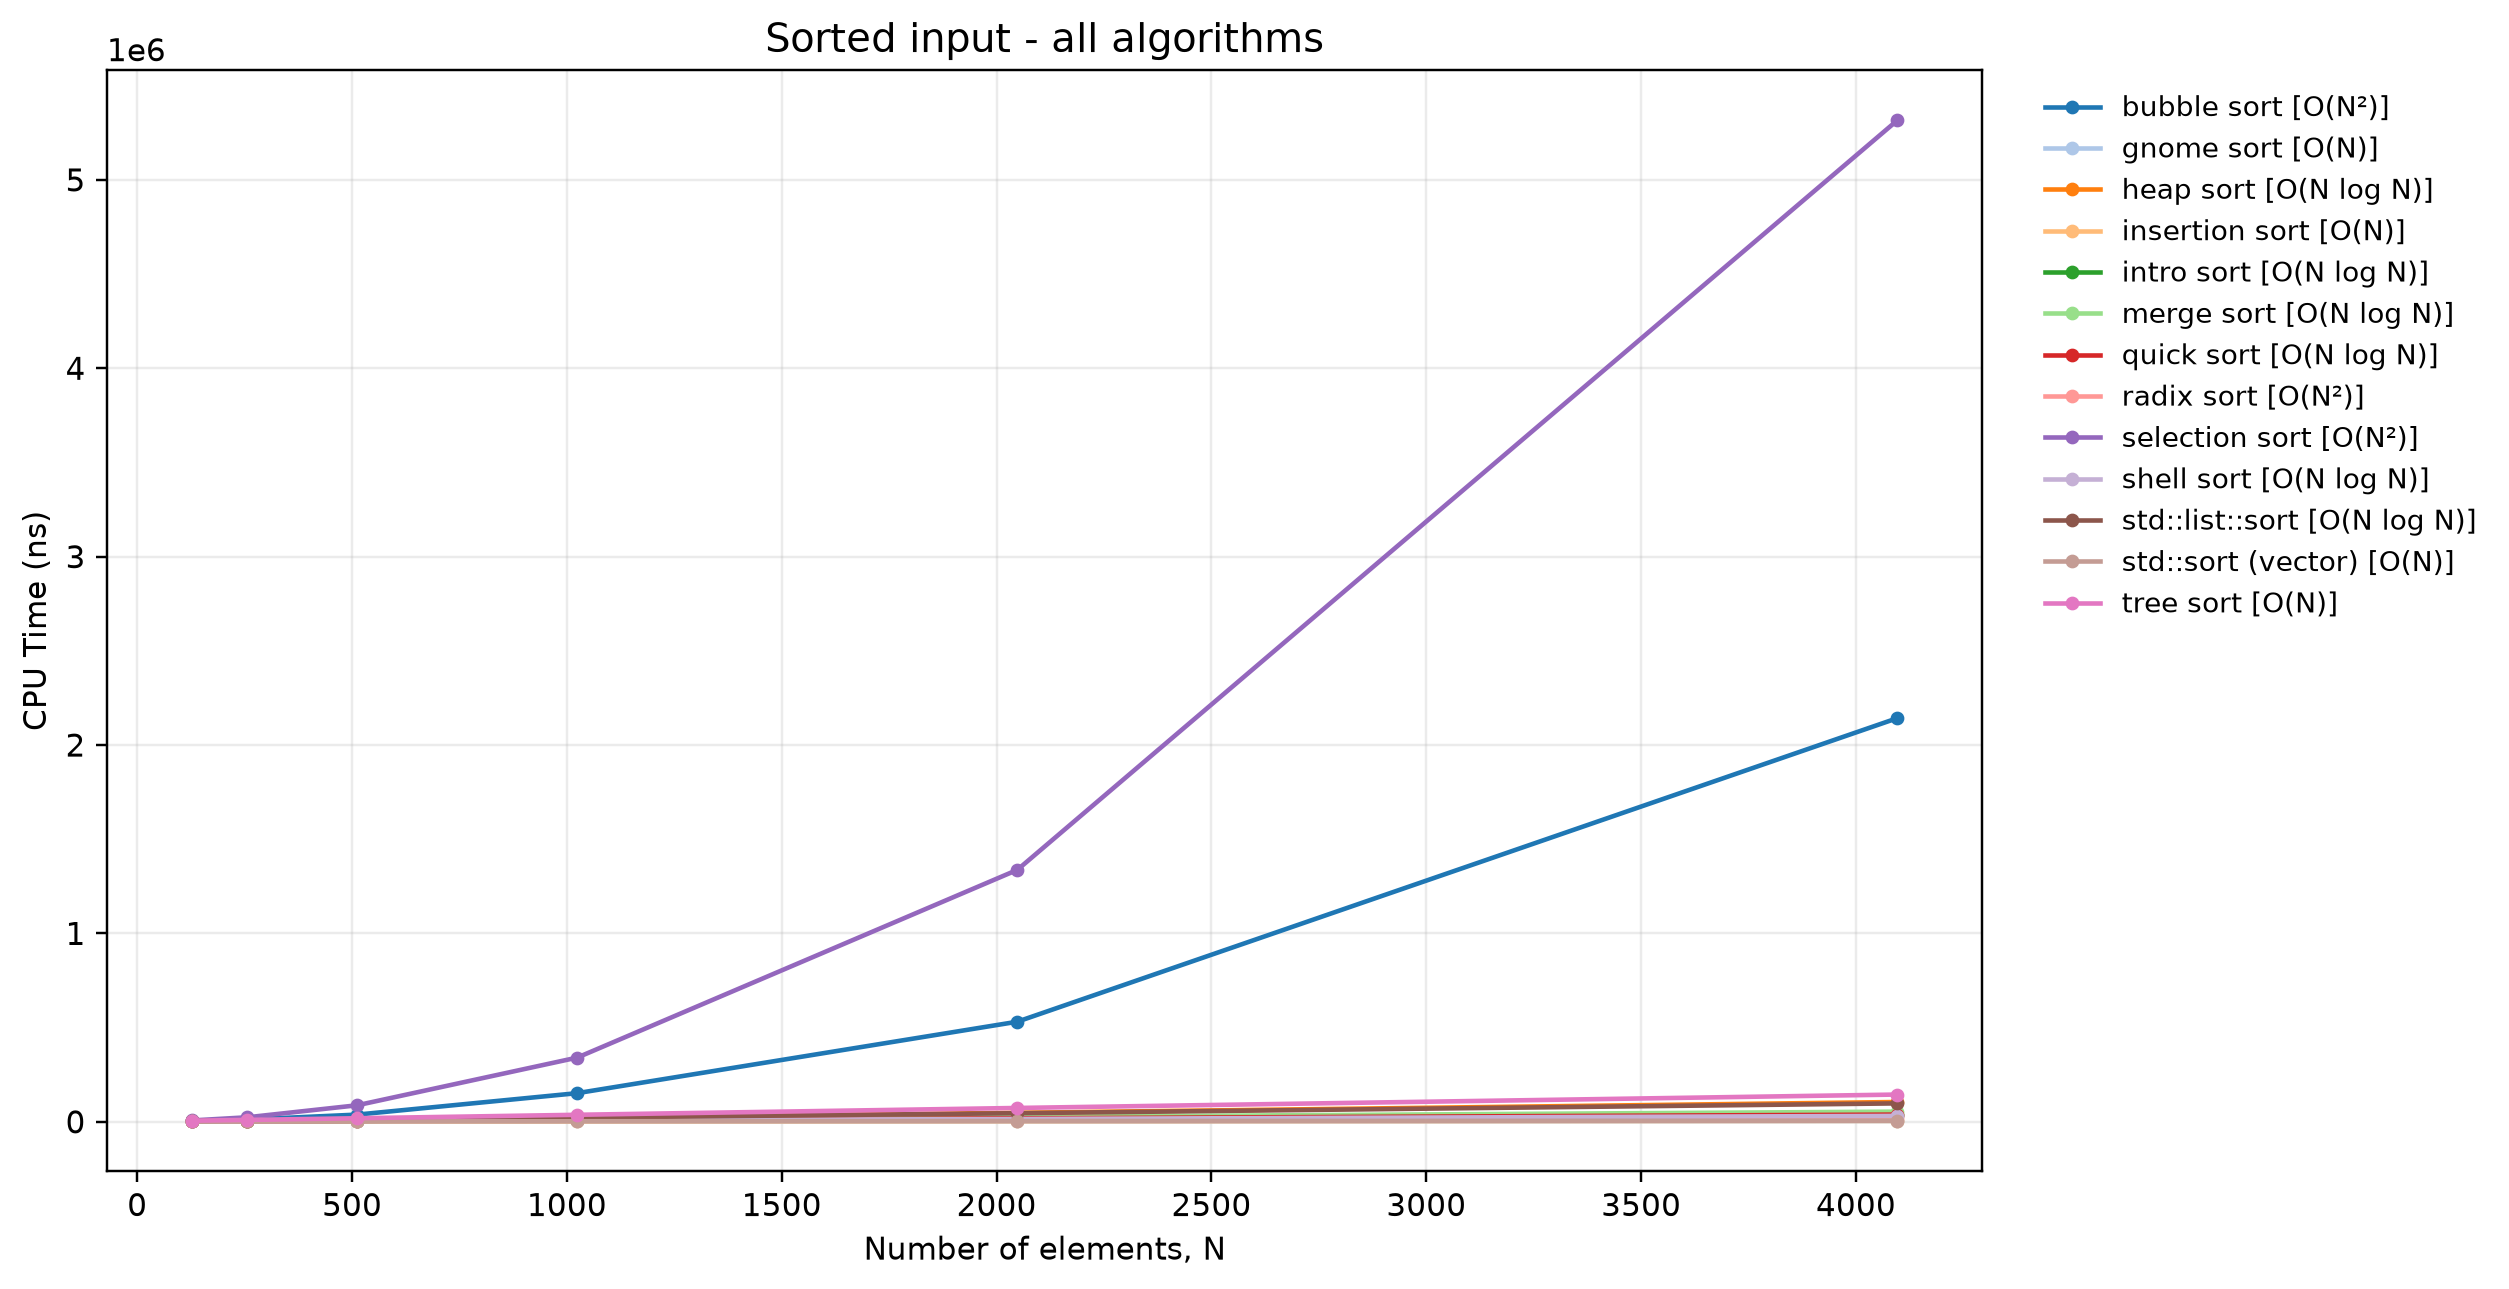
\includegraphics[width=\linewidth]{result/benchmark_overview_sorted_linear.png}
    \caption{\centering{Час сортування впорядкованих даних на лінійних шкалах;\\спільний діапазон вимірювань $N=128$--$4096$}}
    \label{fig:sorted-linear}
\end{figure}

Рисунок~\ref{fig:sorted-loglog} показує ті самі вимірювання на
логарифмічних шкалах. Такий вигляд дає змогу розрізнити швидші алгоритми:
найменший час мають гномове сортування, сортування вставками та
\texttt{std::sort} для вектора. Водночас сортування вибором і бульбашкою
зростають значно швидше за решту.

\begin{figure}[H]
    \centering
    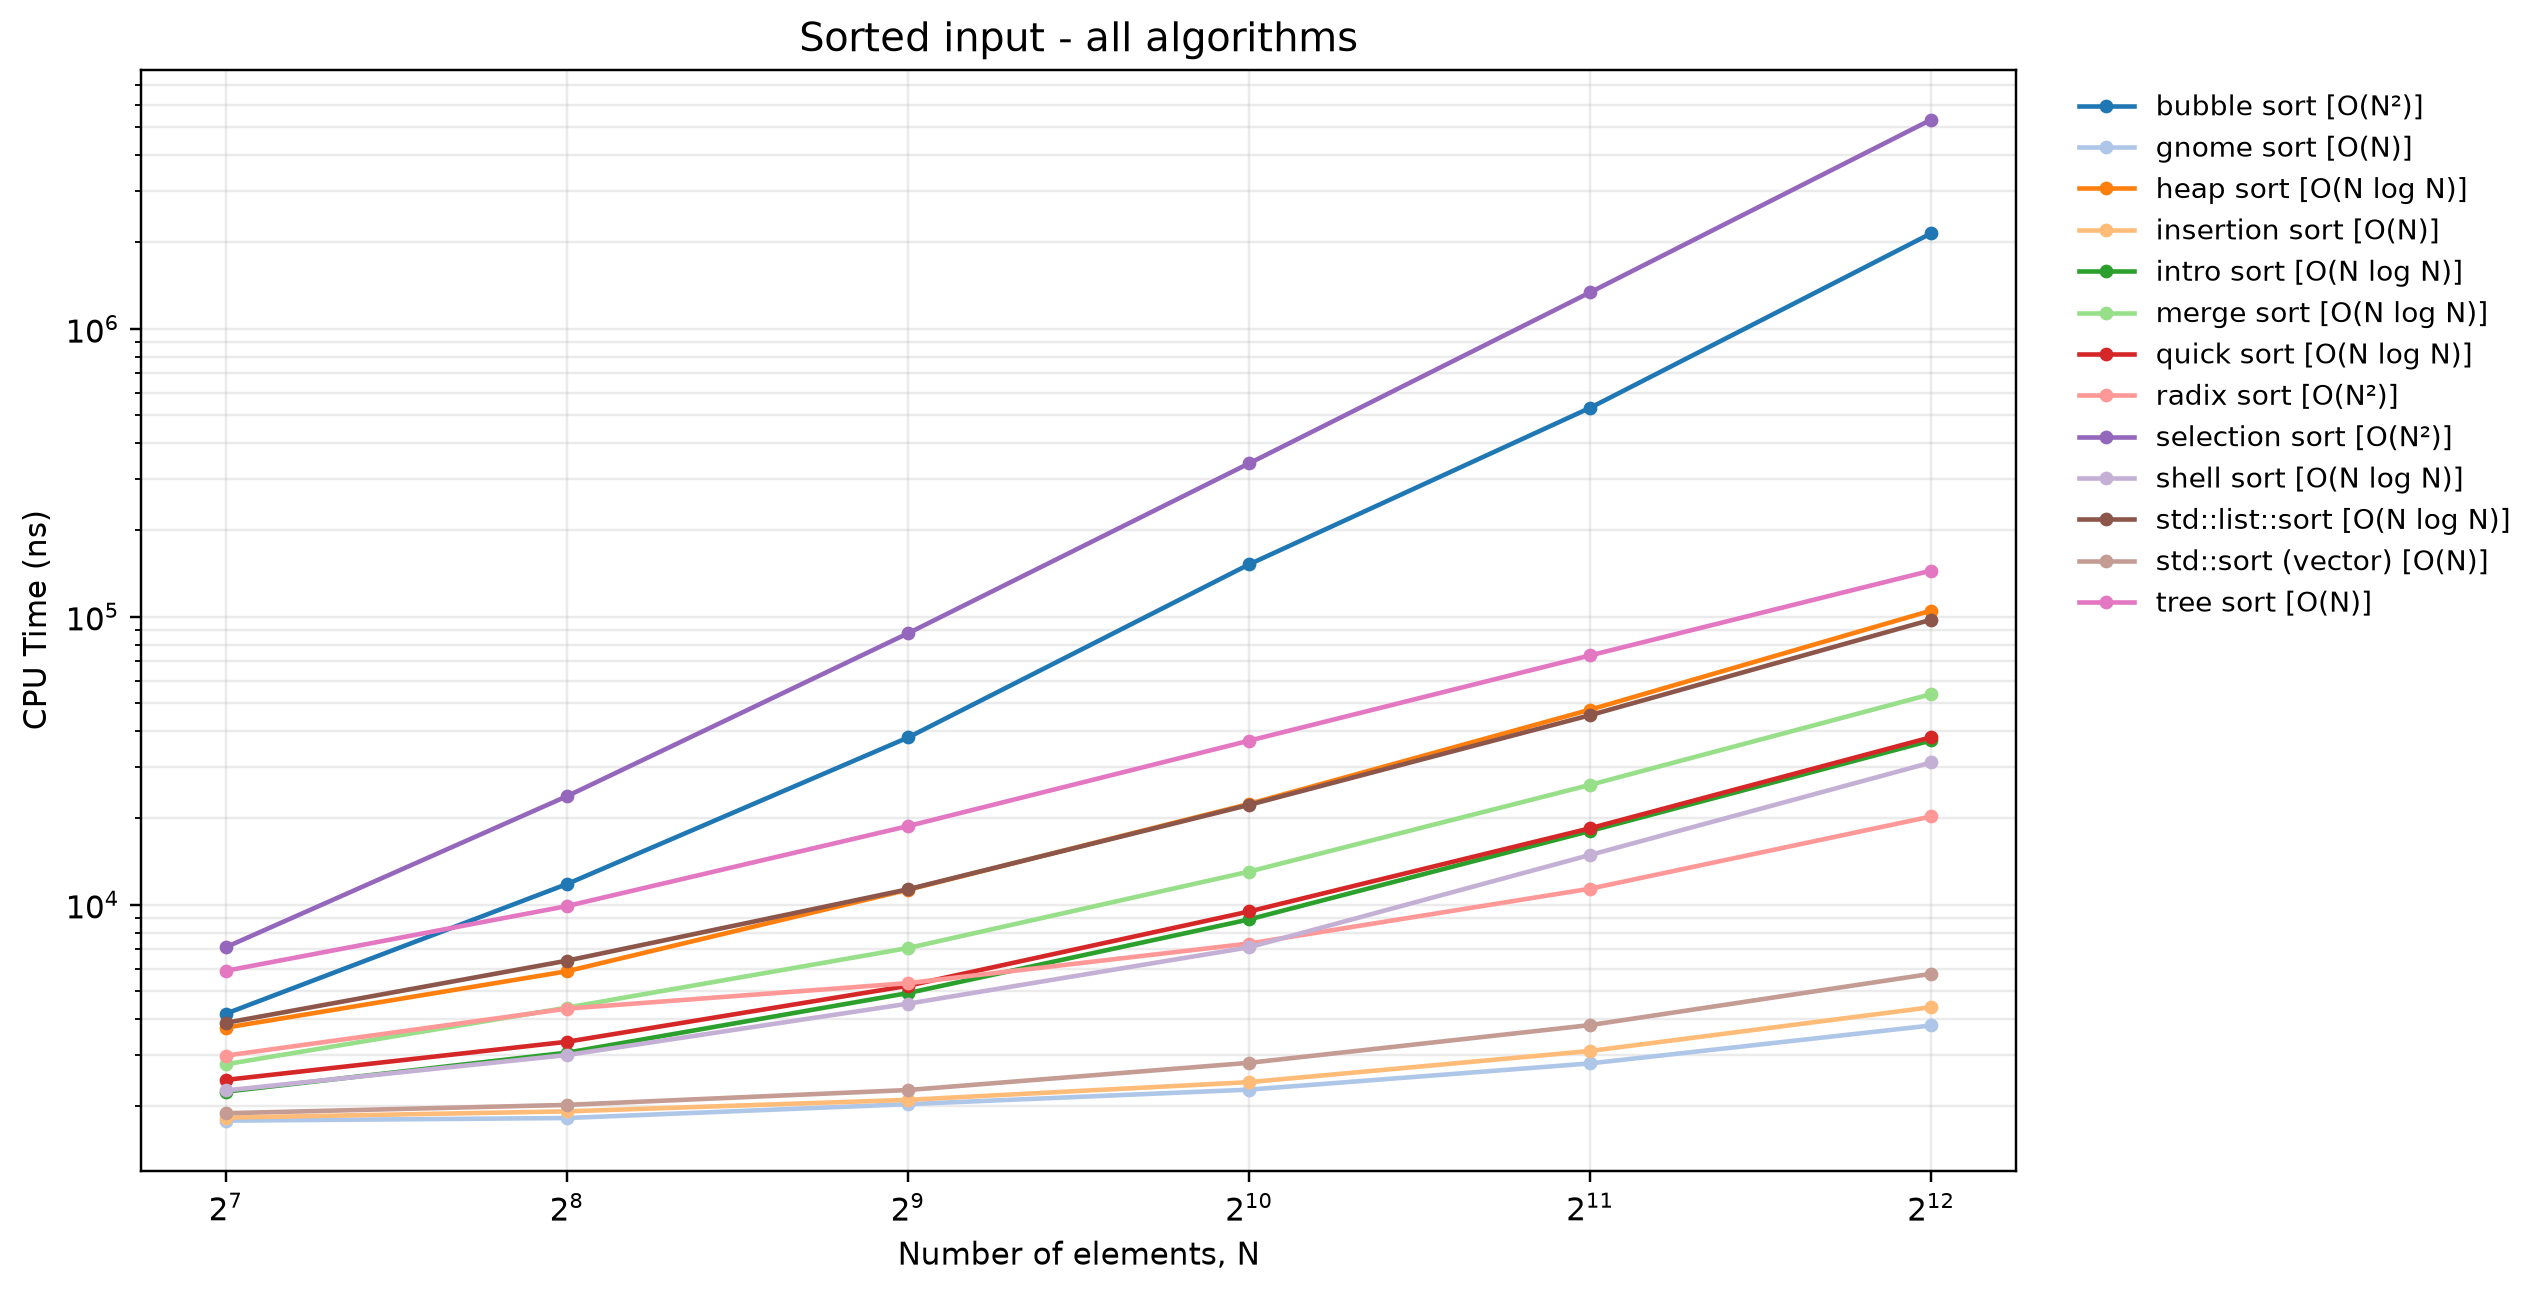
\includegraphics[width=\linewidth]{result/benchmark_overview_sorted_loglog.png}
    \caption{\centering{Час сортування впорядкованих даних на логарифмічних шкалах;\\спільний діапазон вимірювань $N=128$--$4096$}}
    \label{fig:sorted-loglog}
\end{figure}

\subsection{Зворотно відсортовані дані (reverse-sorted)}

На рисунку~\ref{fig:reverse-sorted-linear} найбільший час має гномове
сортування: при $N=4096$ він становить приблизно 11{,}59 мс. Сортування
вибором і бульбашкою мають близькі результати --- 5{,}30 мс і 5{,}24 мс,
а сортування вставками --- 2{,}75 мс. На відміну від впорядкованого входу,
гномове сортування та сортування вставками тут втрачають свою перевагу
й опиняються серед найповільніших.

\begin{figure}[H]
    \centering
    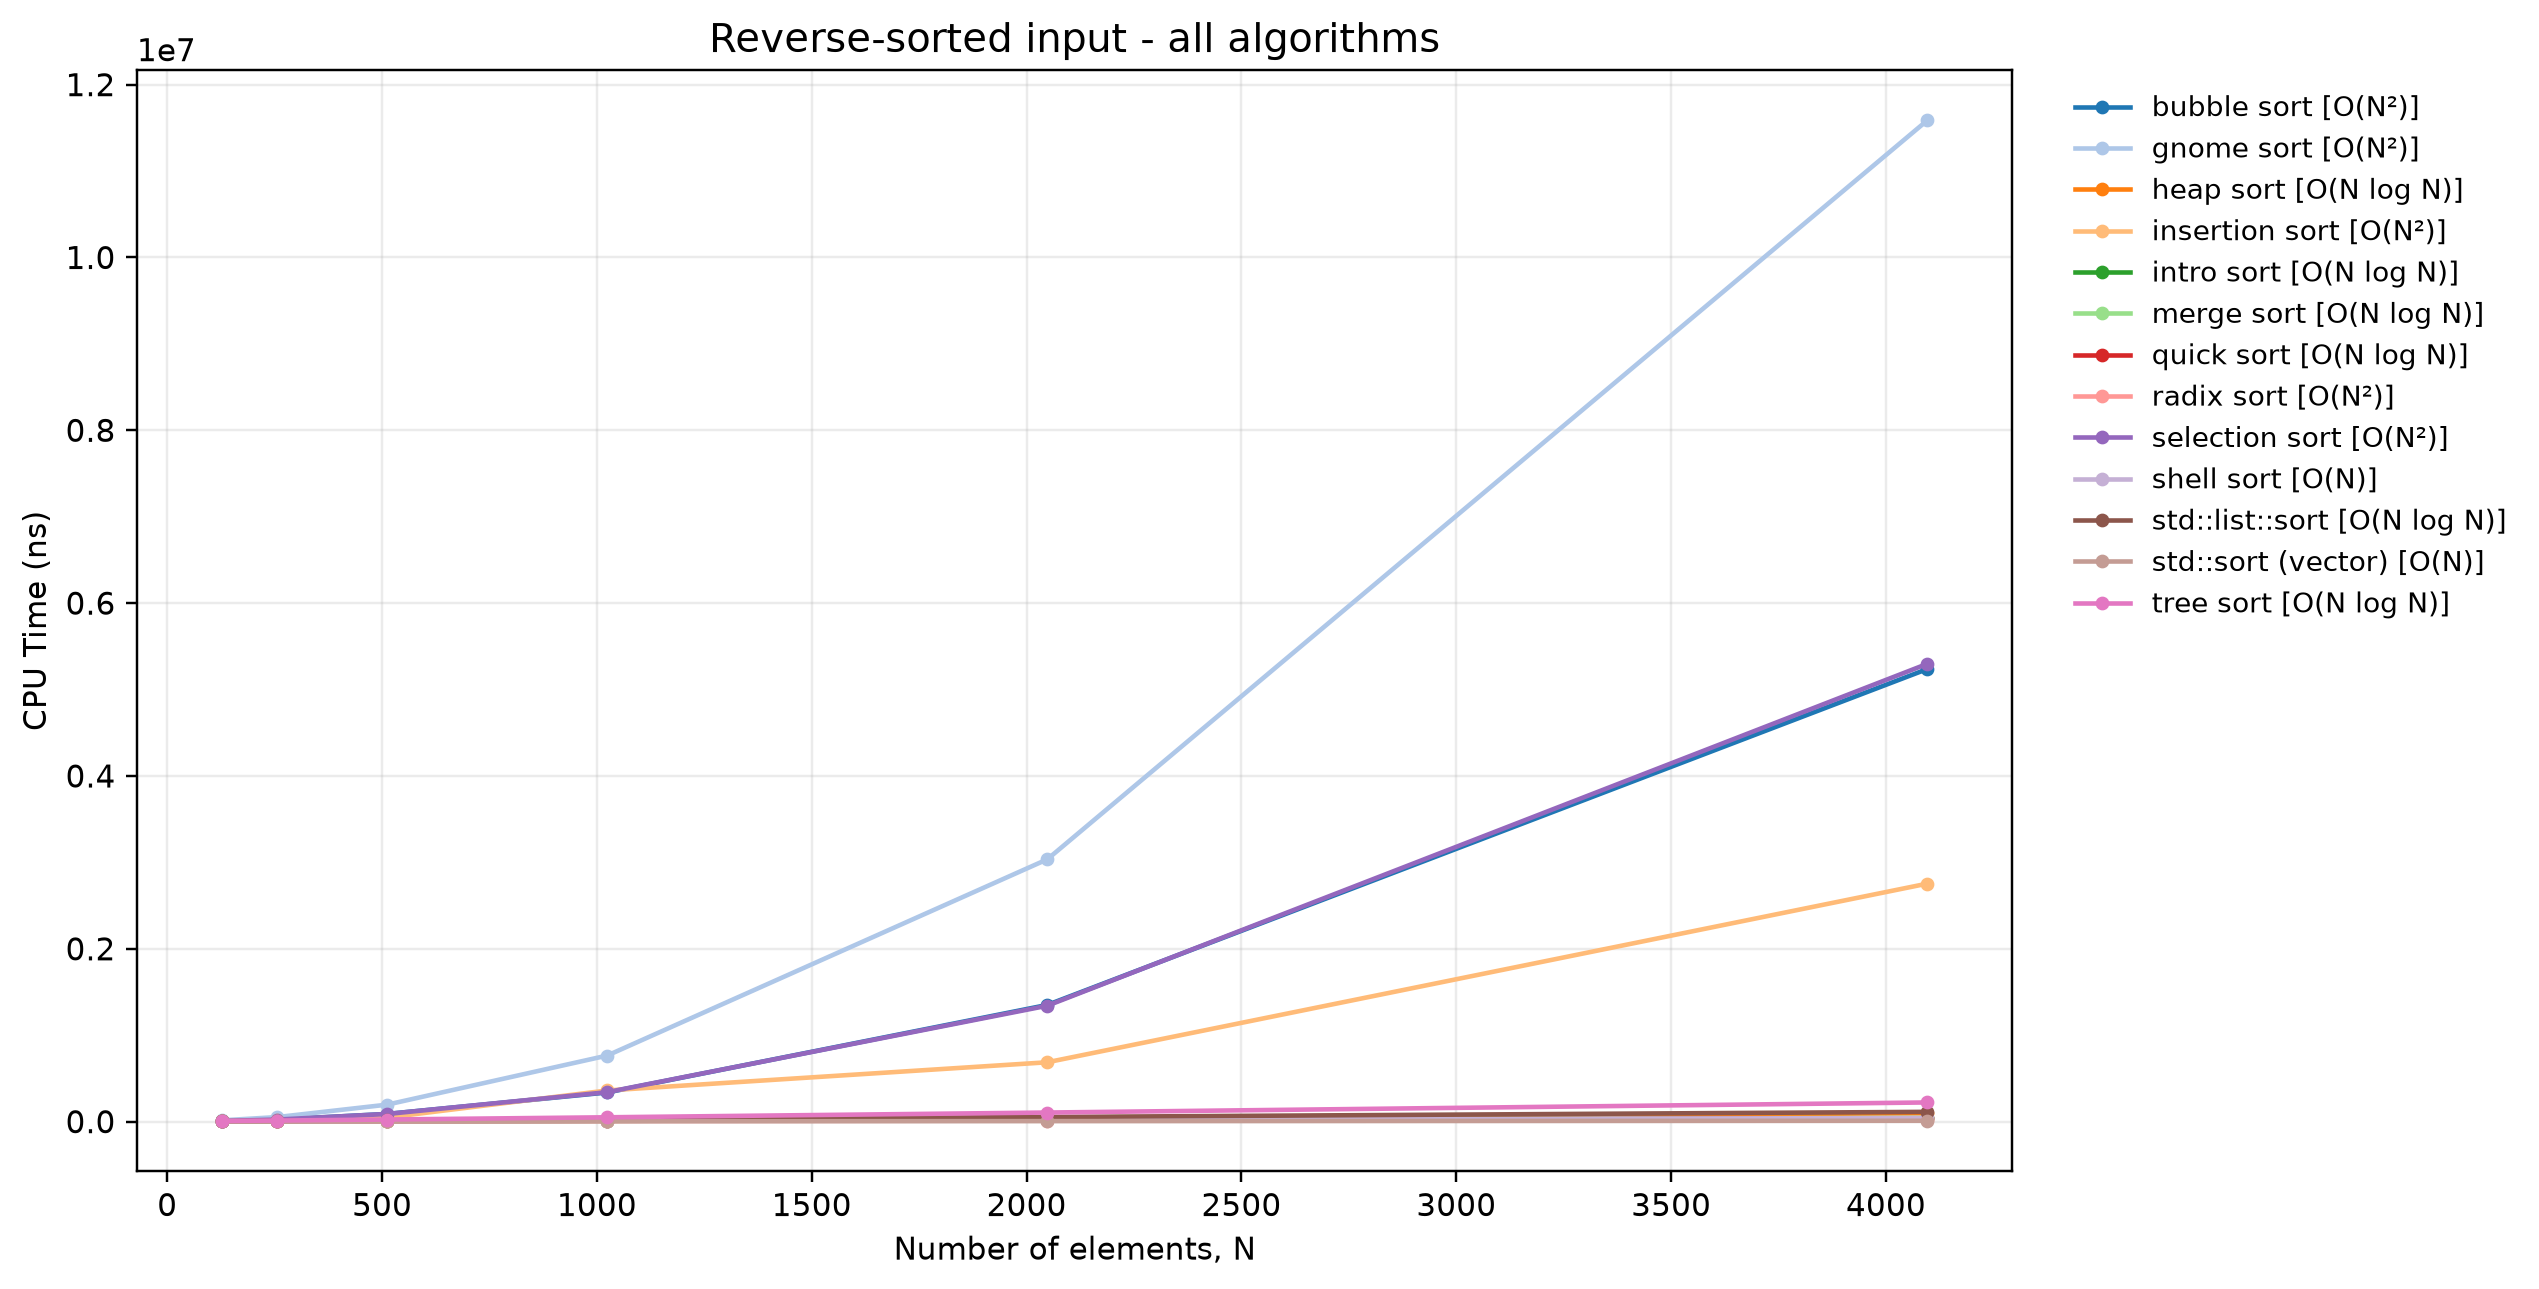
\includegraphics[width=\linewidth]{result/benchmark_overview_reverse_sorted_linear.png}
    \caption{\centering{Час сортування зворотно відсортованих даних на лінійних шкалах;\\спільний діапазон вимірювань $N=128$--$4096$}}
    \label{fig:reverse-sorted-linear}
\end{figure}

На логарифмічному графіку (рис.~\ref{fig:reverse-sorted-loglog}) видно,
що при $N=4096$ найменший час мають \texttt{std::sort} для вектора
(приблизно 9{,}70 мкс) і порозрядне сортування (20{,}59 мкс).
Introsort, швидке сортування, сортування Шелла та злиттям мають близькі
результати --- приблизно 36--43 мкс. Зворотний порядок не є найгіршим
входом для кожного алгоритму: наприклад, у цій точці introsort і швидке
сортування працюють швидше, ніж на випадкових даних.

\begin{figure}[H]
    \centering
    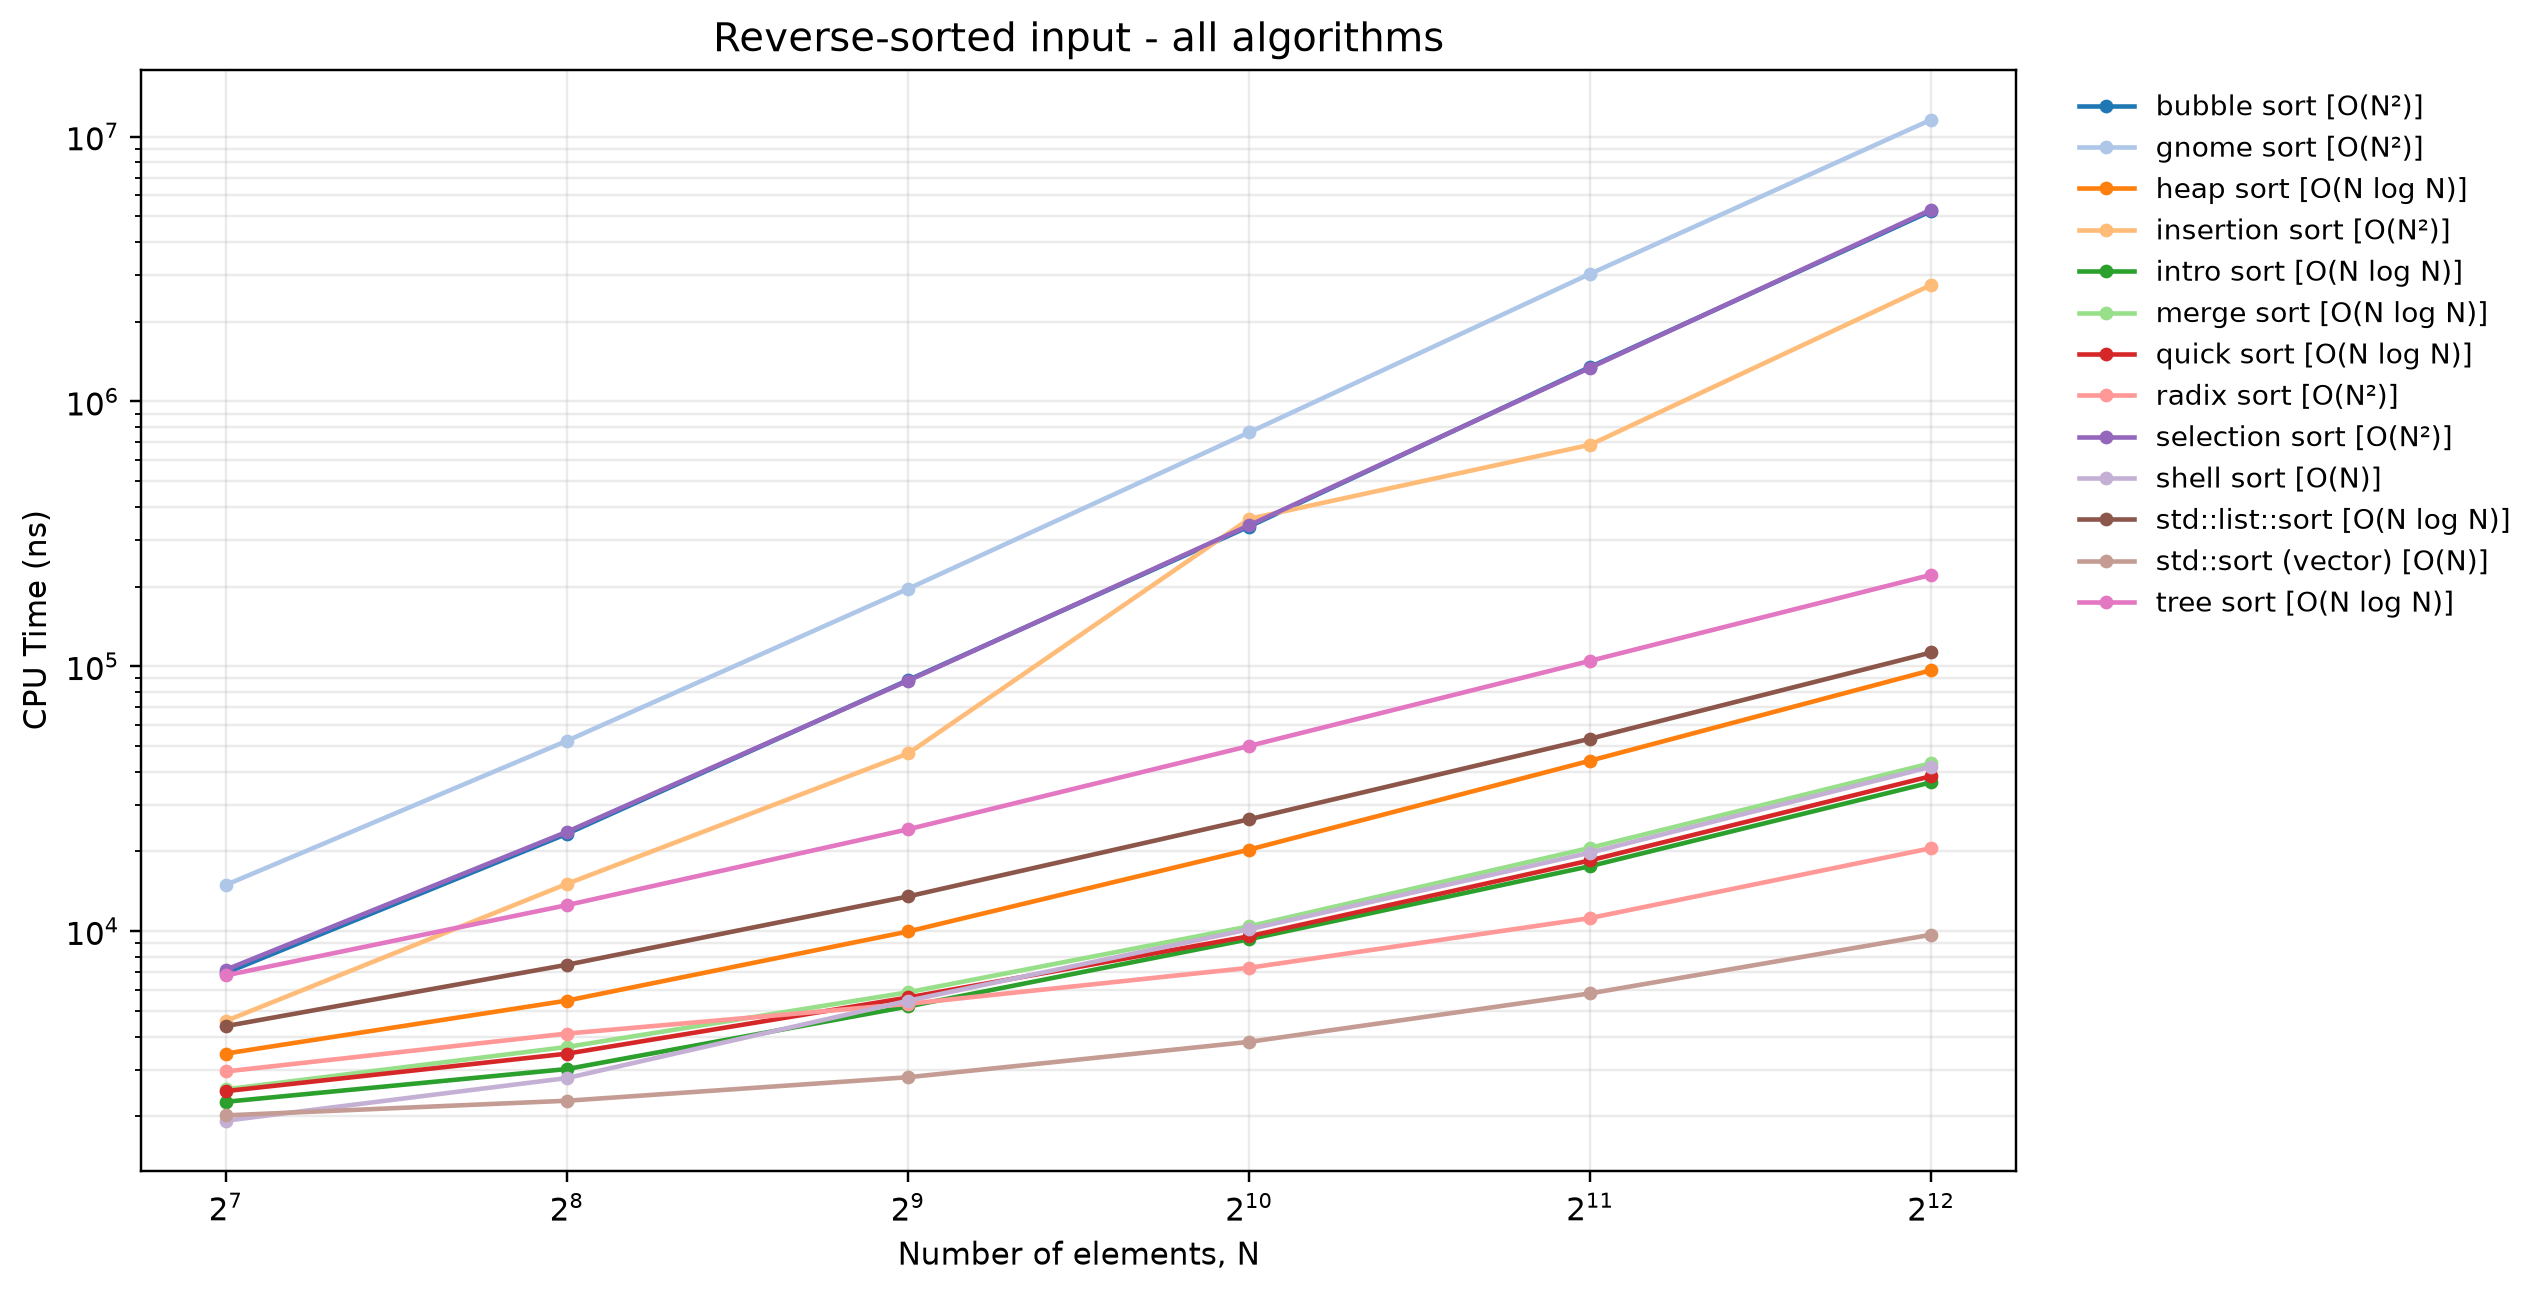
\includegraphics[width=\linewidth]{result/benchmark_overview_reverse_sorted_loglog.png}
    \caption{\centering{Час сортування зворотно відсортованих даних на логарифмічних шкалах;\\спільний діапазон вимірювань $N=128$--$4096$}}
    \label{fig:reverse-sorted-loglog}
\end{figure}

\end{document}
